\documentclass[11pt,a4paper]{article}
\usepackage{fontspec}
\setmainfont{TeX Gyre Pagella}
\newfontfamily\headfont{Inter}[UprightFont=*-ExtraBold,BoldFont=*-ExtraBold,Extension=.otf,Path=/usr/share/fonts/opentype/inter/]
\usepackage[a4paper,margin=2.3cm]{geometry}
\usepackage{graphicx,booktabs,float,caption,array,xcolor,longtable}
\usepackage{xurl}
\usepackage[hidelinks]{hyperref}
\usepackage{titlesec}
\usepackage[round]{natbib}
\usepackage{setspace}
\setstretch{1.05}
\renewcommand{\topfraction}{0.9}
\renewcommand{\bottomfraction}{0.8}
\renewcommand{\textfraction}{0.1}
\renewcommand{\floatpagefraction}{0.75}
\setlength{\parindent}{0pt}
\setlength{\parskip}{0.55em}
\titleformat{\section}{\headfont\Large}{\thesection}{0.8em}{}
\titleformat{\subsection}{\headfont\large}{\thesubsection}{0.8em}{}
\captionsetup{font=small,labelfont=bf}
\urlstyle{same}
\hypersetup{pdftitle={The Nobel Brain Drain},pdfauthor={Tristan Hotham}}

\begin{document}
\begin{center}
{\Large\bfseries The Nobel Brain Drain\par}
\vspace{0.4em}
{\large Where Nobel laureates were born and where they were working when they won,\\1901 to 2026\par}
\vspace{1.2em}
{\large Tristan Hotham\par}
\vspace{0.3em}
{\small Independent researcher\\
ORCID: 0000-0003-4931-9349\\
DOI: https://doi.org/10.5281/zenodo.23857487\par}
\vspace{0.8em}
2026
\end{center}

\begin{quote}
\small
\begin{center}\textbf{Abstract}\end{center}
I compare the birthplaces of Nobel laureates with their affiliations at the time of the award, using the official Nobel Prize API for people, prizes and affiliations and Wikidata for coordinates. Of 760 prizes in physics, chemistry, physiology or medicine and economic sciences from 1901 to 2026 with both a present-day birth country and an affiliation, 237 (31\%) went to people working outside their birth country, a share that has stayed between 24\% and 38\% in every decade. The United States is the only large net gainer: 402 prizes were won by people working there and 271 by people born there, a net gain of 131; 34\% of its prizes went to people born abroad, and it received 57\% of all prizes won outside the laureate's birth country. Germany took 31\% of prizes up to 1932 and 7\% since 1933; 10\% of German-born laureates up to 1932 were working abroad, against 49\% since. Japan rose from 5 science laureates in the twentieth century to 22 since 2000, most of them working in Japan. Nine of the ten institutions with most prizes are American. Women won 3.8\% of prizes to people before 1960 and 20\% in the 2020s so far. Affiliation at the award is not always where the winning work was done, and birth country is not nationality; I report both caveats with the results.

\textbf{Keywords:} Nobel Prize; scientific migration; brain drain; science history; Wikidata; open data; flow maps
\end{quote}

\section{Introduction}
Nobel prizes are a famously narrow measure of science, but a well recorded one, and they have long been used to study where scientific excellence is produced and where it moves \citep{zuckerman,schlagberger}. The prizes are claimed by places twice over: by the country where a laureate was born and by the institution where they worked. The gap between the two is a small, visible piece of the history of scientific migration: the European emigration of the 1930s \citep{medawar}, the post-war pull of American universities, and more recent flows from Asia.

The Nobel Prize Outreach organisation publishes an open API that records, for every prize, the laureate's birthplace and their affiliations at the time of the award \citep{nobelapi}. Wikidata adds coordinates for birthplaces and employers \citep{wikidata}. Together they allow a simple, fully reproducible map of every laureate's journey from birthplace to prize, and a country-by-country account of gains and losses. This paper sets out the data and method, then reports the net balance of countries, the role of the United States, Germany before and after 1933, the rise of Japan, the leading institutions, the share of women and the share born abroad over time. It accompanies an interactive map (\url{https://maps.tristanhotham.com/nobel-brain-drain/}).

\section{Data}
\textbf{Nobel Prize API.} The API (version 2.1), retrieved in 2026, lists 1,028 laureates, 28 of them organisations. For each person it gives a known name, sex, date and place of birth (city and country as named at the time, and as named now, with coordinates for the present-day city where available), and for each prize the year, category, share, motivation and either the affiliations at the time of the award (name, city, country) or, mostly for Peace and Literature, the country of residence. I treat the API as authoritative for names, prizes, years and affiliations. The downloaded file contains no licence statement; I credit Nobel Prize Outreach and note that the terms of use on nobelprize.org should be checked before reusing the derived laureate list.

\textbf{Wikidata.} A query through QLever \citep{qlever} returned 2,075 rows for 666 laureates of the physics, chemistry and medicine prizes, with prize, year, place of birth and its coordinates, and employers (P108) with their coordinates or headquarters coordinates. The affiliation property (P1416) came back empty, so employers are used to place affiliations. Wikidata is CC0.

\textbf{Other sources.} Natural Earth \citep{naturalearth} countries and populated places; and Wikipedia's ``List of Nobel laureates by university affiliation'' (revision 1381233532, CC BY-SA 4.0), used only to cross-check institution counts.

\begin{table}[tbp]\centering\small\caption{From sources to the flow analysis.}\label{tab:pipe}\begin{tabular}{p{10.5cm}r}\toprule Step & Count\\\midrule
Laureates in the Nobel Prize API & 1,028\\
\quad of which organisations (excluded) & 28\\
Prizes awarded to people (records) & 1,005\\
\quad physics, chemistry, medicine, economics & 769\\
\quad\quad with no affiliation in the API & 7\\
\quad\quad with no birthplace in the API & 2\\
\quad\quad in the flow analysis & 760\\
\quad peace and literature & 236\\
\quad\quad with a country of residence & 224\\
Wikidata rows (physics, chemistry, medicine) & 2,075\\
\quad people & 666\\
\quad matched to API records (identifier, prize and year) & 666\\
\quad matched by name, prize and year only & 2\\
\bottomrule\end{tabular}\end{table}

\section{Methods}
\subsection{Records and scope}
The unit is a prize awarded to a person: 1,005 records for 1,000 people, since 5 people won twice. Organisations are excluded. The flow analysis covers the four prizes for which the API gives affiliations: 769 records, of which 7 have no affiliation (Marie Curie in 1903, Hayek and Myrdal in 1974 and four others) and 2 no birthplace, leaving 760 (99\%). Peace and Literature laureates are analysed separately by country of residence. Award decades run from the 1900s (1901 to 1909) to the 2020s (2020 to 2026).

\subsection{Matching}
Wikidata people were matched to API records by Wikidata identifier, requiring the same prize and year. All 668 physics, chemistry and medicine records matched: 666 by identifier, two by normalised name, prize and year where Wikidata holds a duplicate item. Matching by name alone would have found only 492, because the API's known names often differ from Wikidata labels (``Sir Alexander Fleming''). Two Wikidata rows matched nothing: an item without an English label and the fictional laureate Sheldon Cooper.

\subsection{Places and countries}
Birth and work countries are the API's present-day countries. Birthplaces are placed at Wikidata's coordinates when they lie within 100 km of the API's city point or inside the API's birth country (664 records); otherwise at the API's city point (334), a Natural Earth town of the same name (1) or the country's label point (6). Where both points exist their median distance is 0.5 km; the largest disagreements are namesake towns in the API (Cluny in France for John Macleod, born in Cluny, Scotland). 99\% of placed birthplaces fall inside the API's present-day country on Natural Earth outlines.

The primary affiliation is the first the API lists that has a place; the Howard Hughes Medical Institute and the LIGO/VIRGO Collaboration are listed without a city, so the university listed beside them is used. 83 records list several affiliations and 19 list affiliations in more than one country. The affiliation is placed at a Wikidata employer of the same person whose name matches it (similarity, containment or shared distinctive words) and whose point lies within 60 km of the API's city (474 of 760); otherwise at the API's city point (284) or a hand-set point (2). Table~\ref{tab:methods} summarises the methods; every row of the released data carries them.

\begin{table}[tbp]\centering\small\caption{How points were placed: birthplaces of all records, workplaces of the flow analysis.}\label{tab:methods}\begin{tabular}{p{10.5cm}r}\toprule Method & Records\\\midrule
\textbf{Birthplace} & \\
Wikidata birthplace coordinates & 664\\
Nobel API present-day city point & 334\\
Natural Earth town of the same name & 1\\
Country label point (birthplace vague) & 6\\
No birthplace & 2\\
\textbf{Workplace (flow analysis)} & \\
Wikidata employer matched to the affiliation & 474\\
Nobel API city point (city centroid) & 284\\
Hand-set point & 2\\
\bottomrule\end{tabular}\end{table}

\subsection{Measures}
A record is \emph{born abroad} when the birth country differs from the country of the primary affiliation. A country's \emph{net gain} is the number of records affiliated there minus the number born there. For the section on Germany, a laureate is German-born when the API names the birth country at the time of birth as Germany or a German state (Prussia, Bavaria, Mecklenburg and others), whatever the present-day country. Institutions are counted for every listed affiliation, as on the Wikipedia list, with campuses of the University of California kept apart and the Rockefeller Institute counted as Rockefeller University.

\section{Results}
\subsection{The map}
Figure~\ref{fig:map} draws every born-abroad record as a curve from birthplace to workplace. The dominant feature is the movement from Europe to the north-eastern United States and California; Figure~\ref{fig:europe} shows the denser web inside Europe. Overall 31\% of records are born abroad. The four subjects are similar: chemistry 34\%, physics 32\%, economics 31\% and medicine 28\%. Table~\ref{tab:flows} lists the largest country pairs.

\begin{figure}[tbp]\centering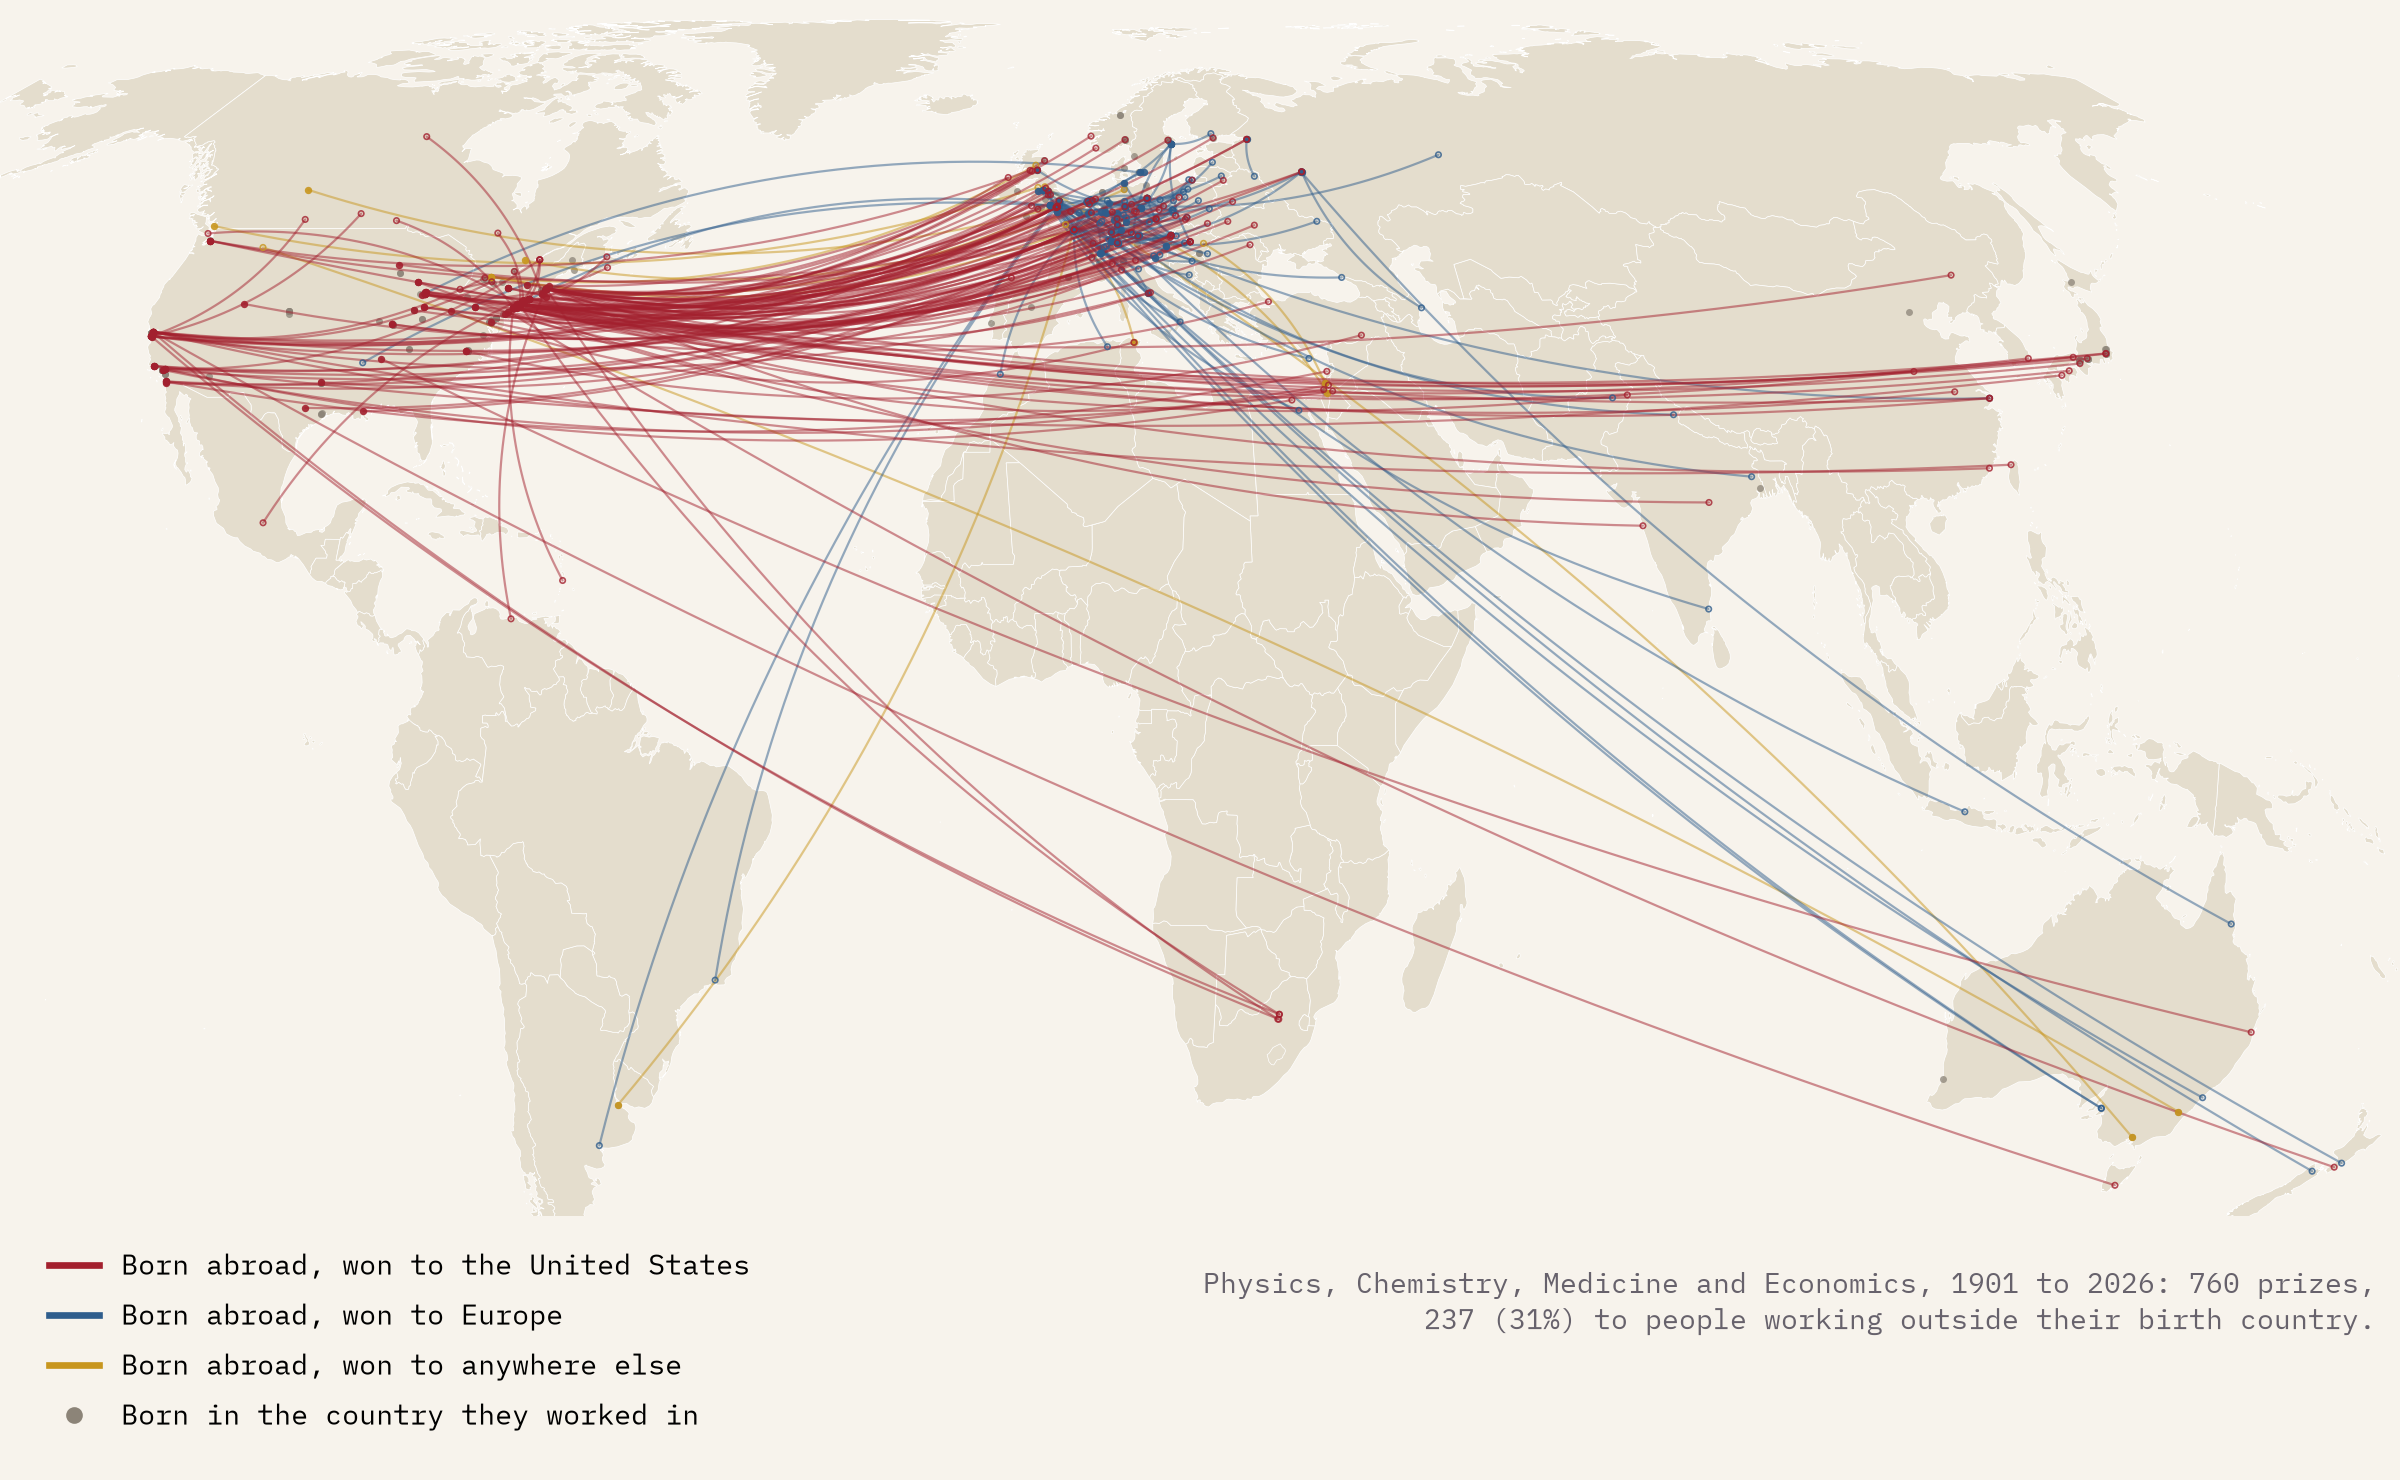
\includegraphics[width=\textwidth]{f_flowmap.png}
\caption{Born-abroad Nobel laureates in physics, chemistry, medicine and economics, from birthplace to affiliation at the award, coloured by where they won. Grey dots: laureates who won in their birth country. Equal Earth projection.}\label{fig:map}\end{figure}

\begin{figure}[tbp]\centering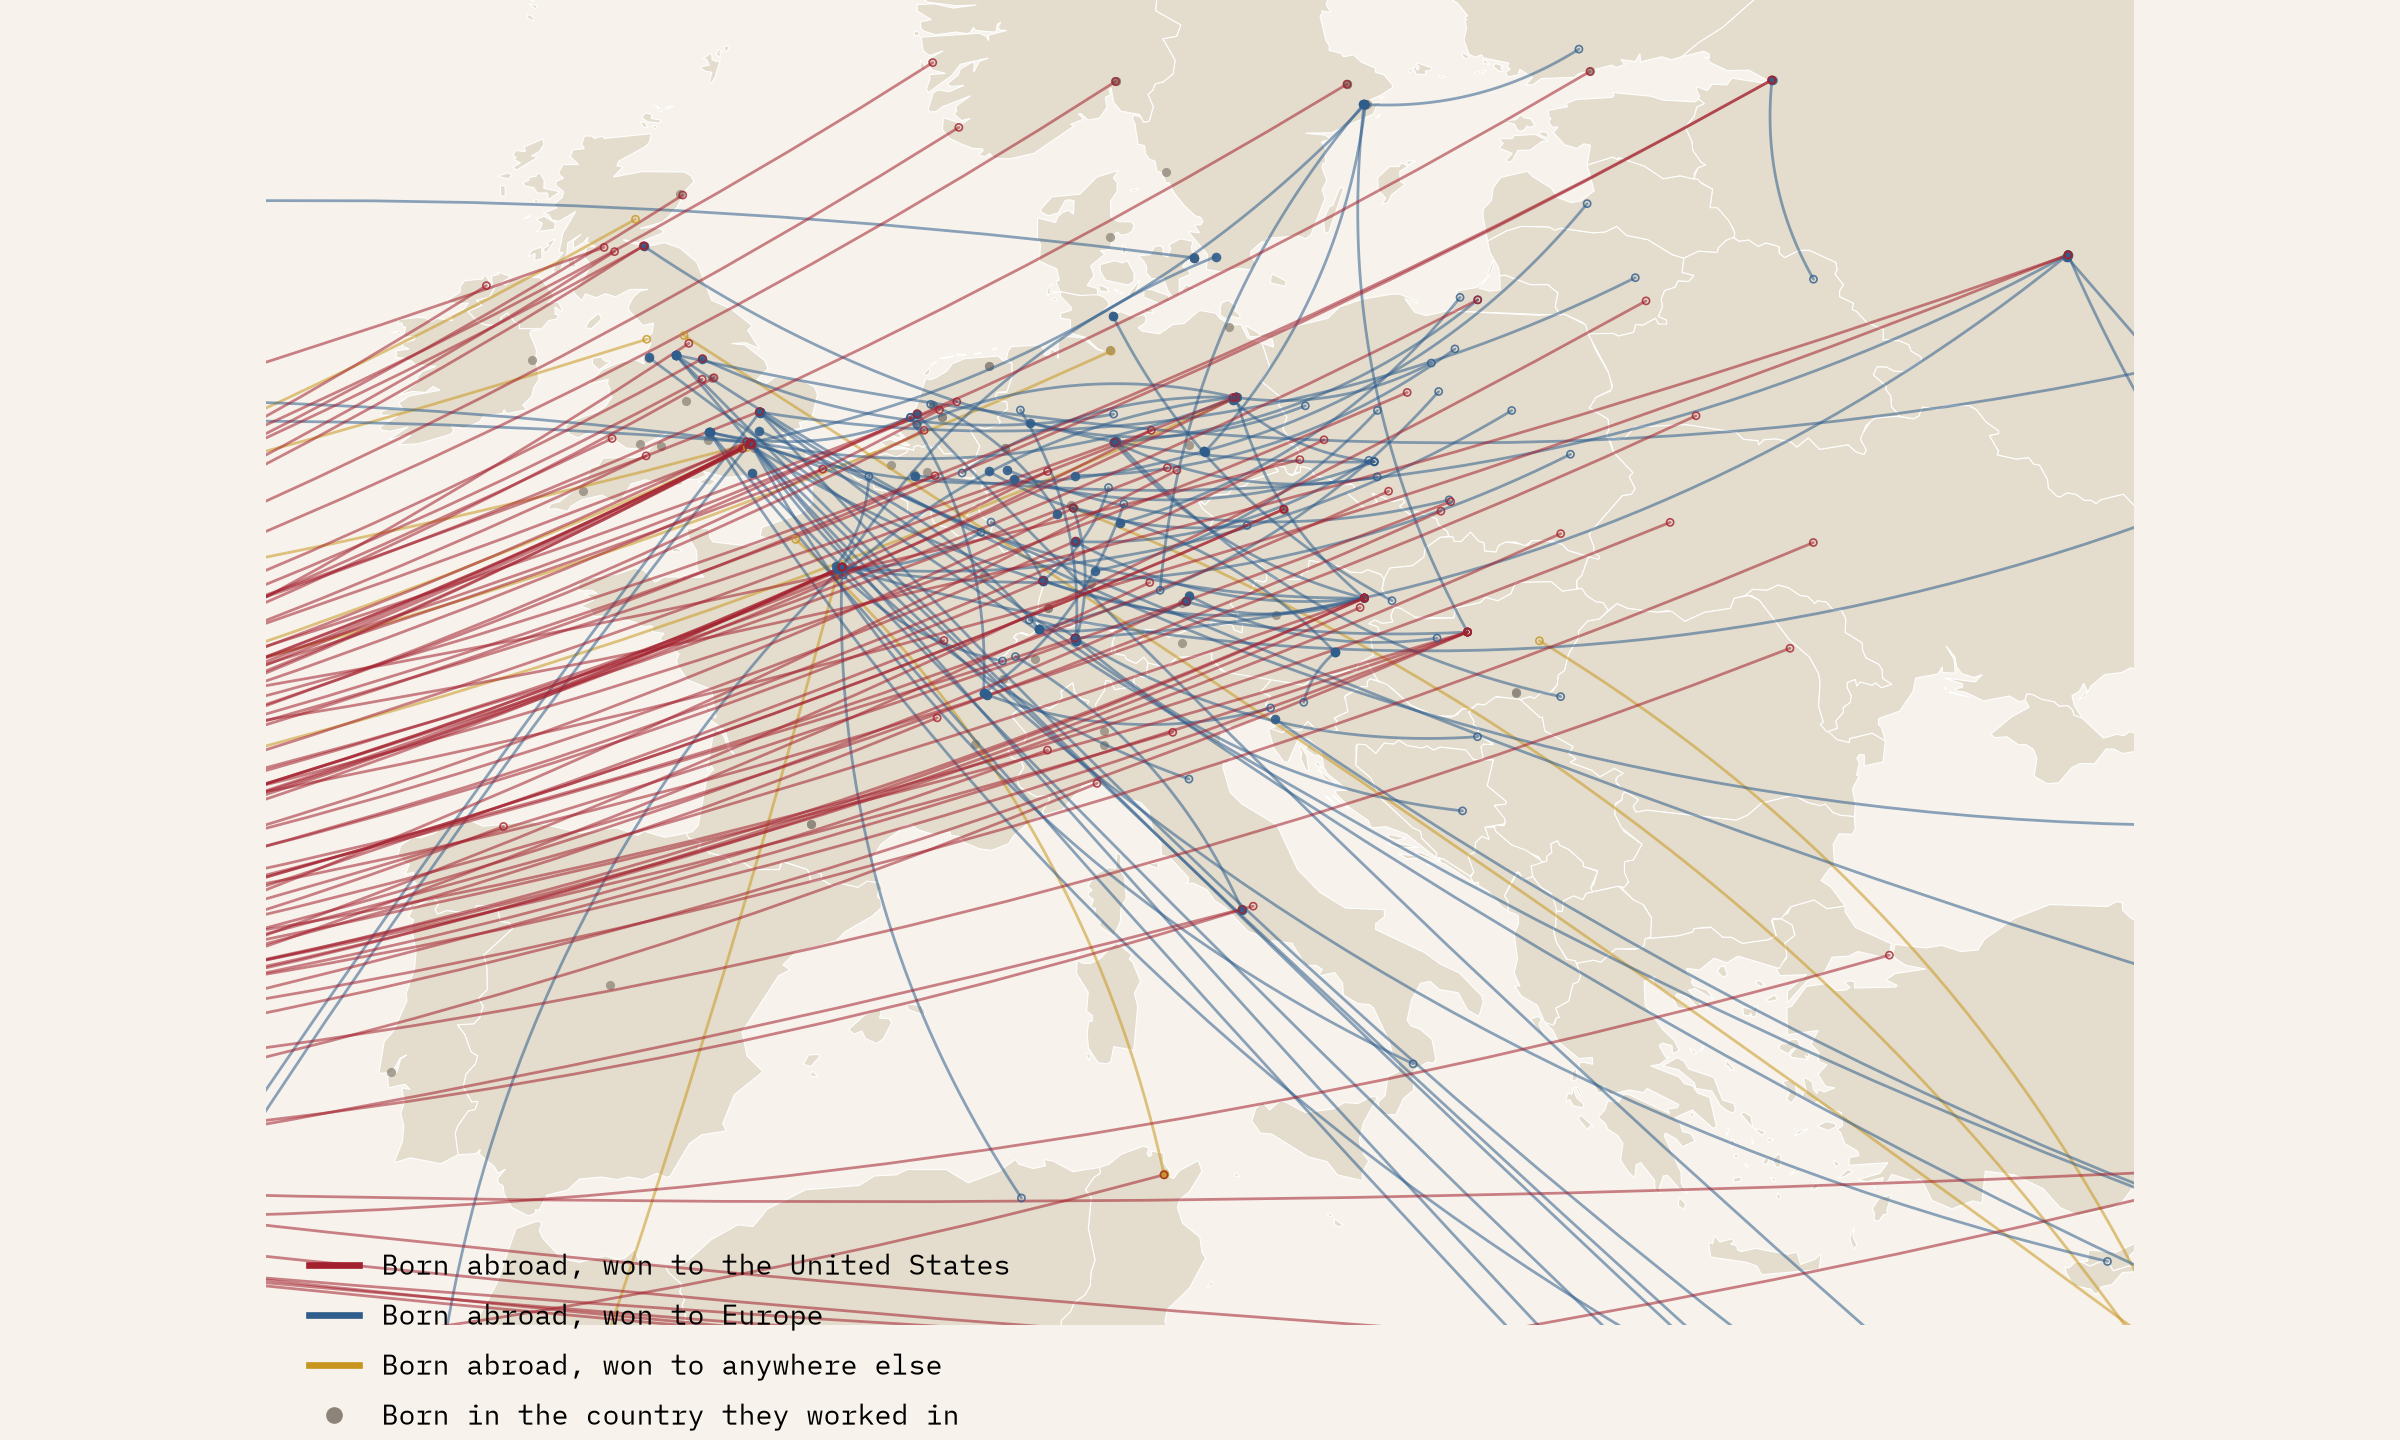
\includegraphics[width=\textwidth]{f_europe.png}
\caption{The same flows around Europe.}\label{fig:europe}\end{figure}

\begin{table}[tbp]\centering\small\caption{The largest flows from birth country to country of affiliation (present-day borders).}\label{tab:flows}\begin{tabular}{llr}\toprule Born in & Won in & Prizes\\\midrule
United Kingdom & United States & 20\\
Canada & United States & 15\\
Germany & United States & 12\\
Poland & Germany & 9\\
France & United States & 8\\
Japan & United States & 7\\
Poland & United States & 6\\
China & United States & 6\\
Russia & United States & 5\\
Italy & United States & 5\\
South Africa & United States & 4\\
Austria & United States & 4\\
Austria & Germany & 4\\
Hungary & United States & 4\\
United Kingdom & Canada & 4\\
\bottomrule\end{tabular}\end{table}

\subsection{Net gain and loss}
Only 5 countries have a positive balance (Figure~\ref{fig:net}, Table~\ref{tab:countries}): the United States (+131), Switzerland (+9), the United Kingdom (+2), Denmark and Sweden (+1 each). The largest losses are Poland (-19), Canada (-9), and Austria, Hungary, the Netherlands and Russia (-8 each). Poland's figure is largely a border effect: 14 of its 19 laureates were born in what was then Germany, and 8 won in Germany. Germany on present-day borders balances exactly (74 born, 74 won there). The United Kingdom both sends and receives: 26 British-born laureates won abroad, 20 of them in the United States, and 28 laureates born elsewhere won in Britain.

\begin{figure}[tbp]\centering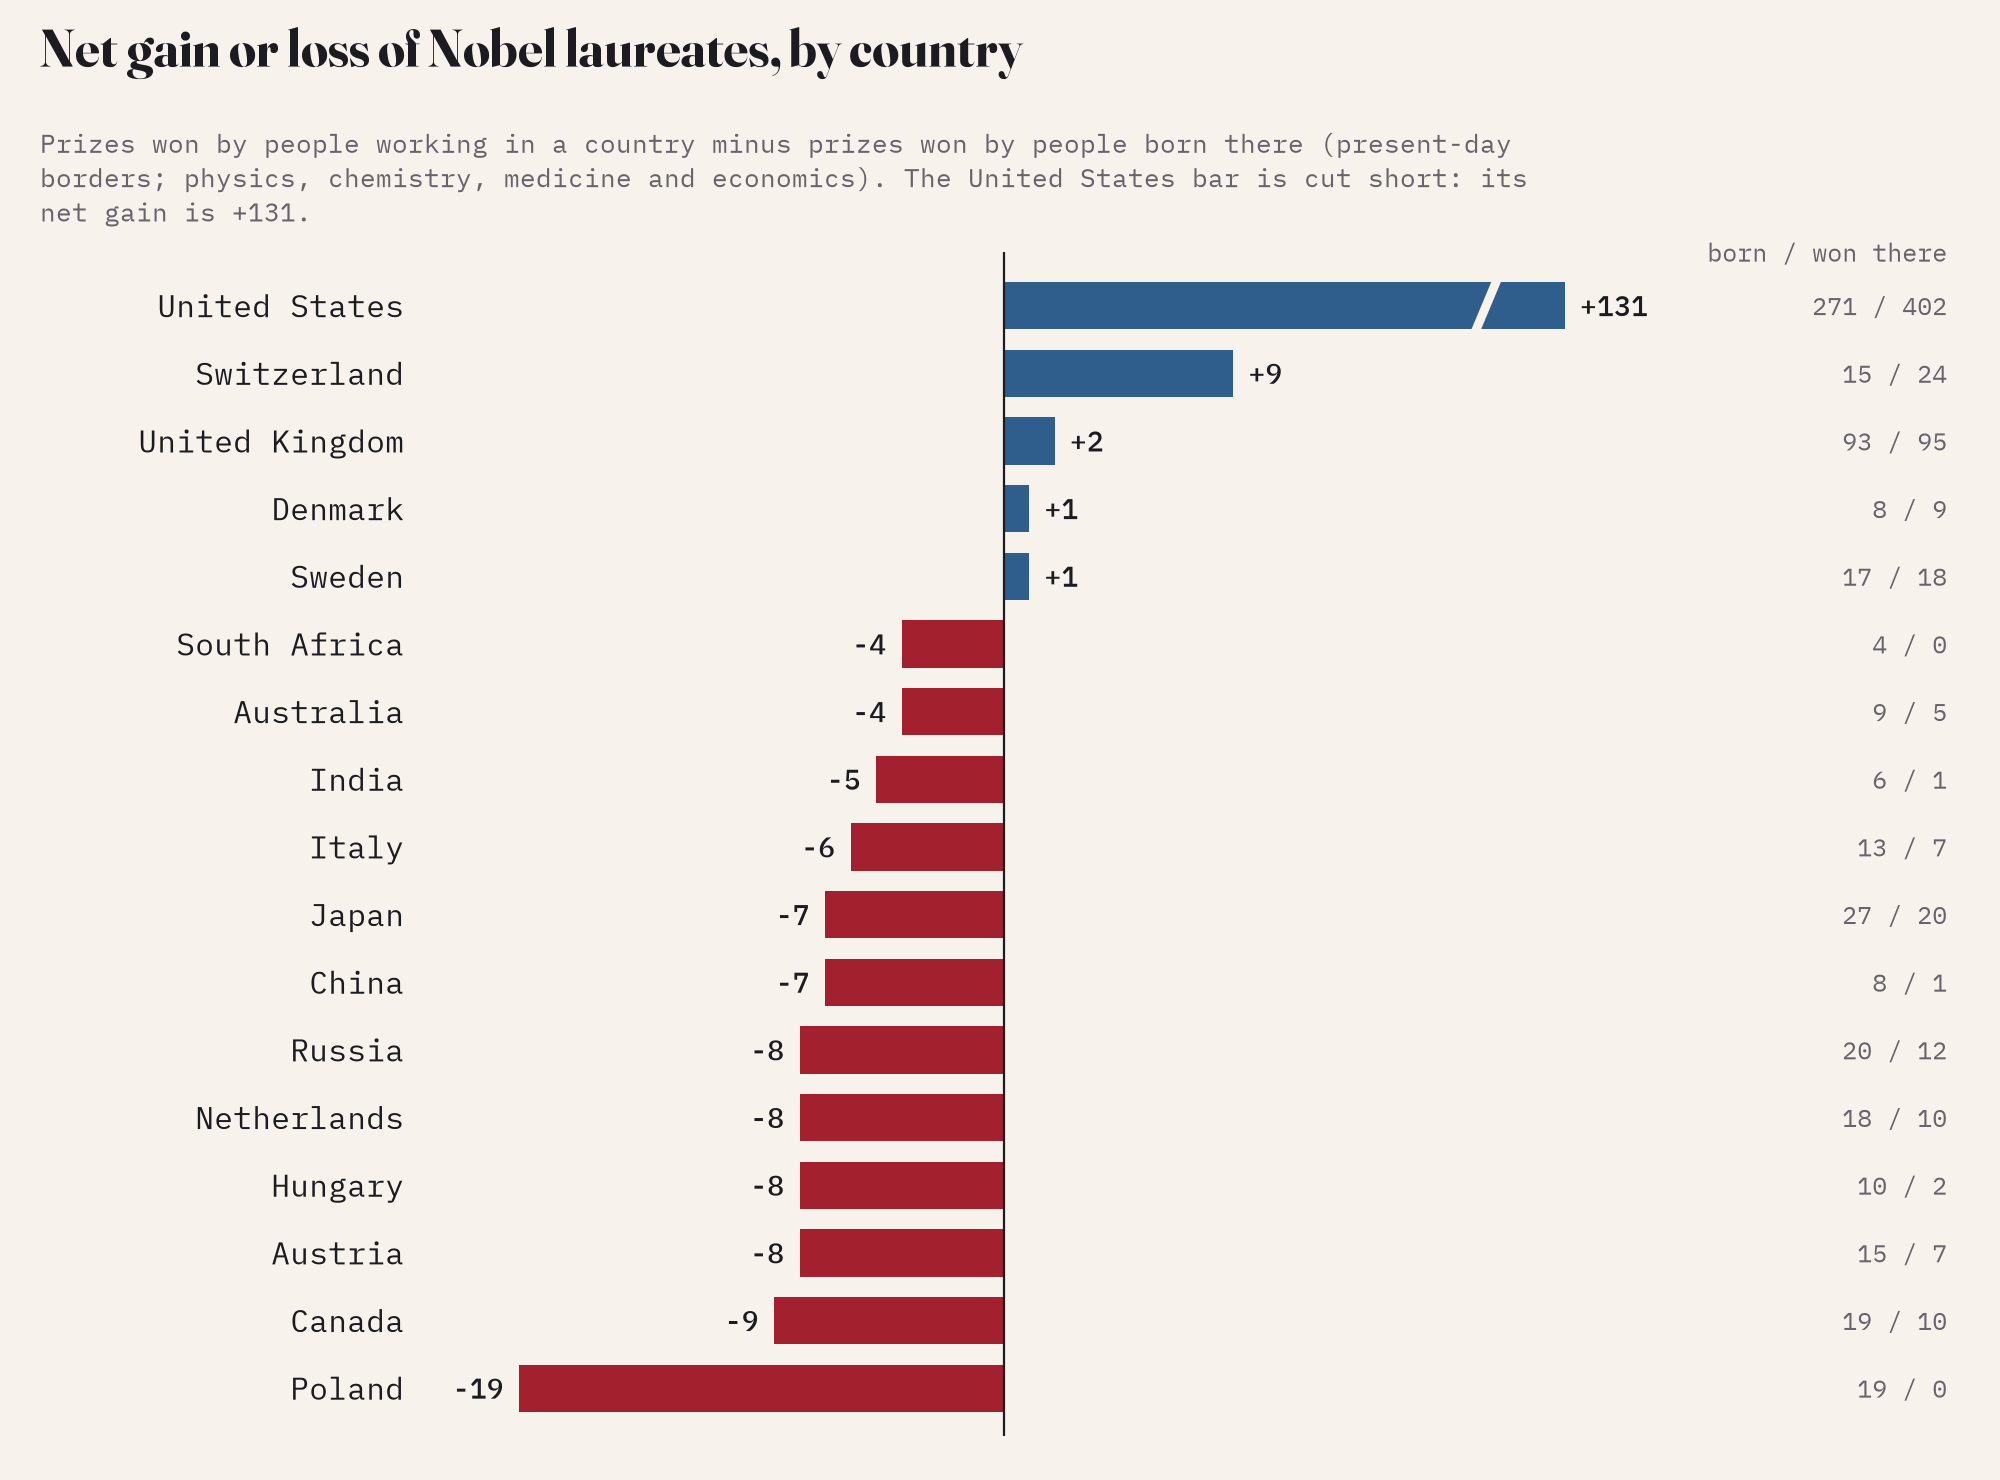
\includegraphics[width=.86\textwidth]{f_net.png}
\caption{Net gain or loss by country: records affiliated in a country minus records born there. The United States bar is truncated.}\label{fig:net}\end{figure}

\begin{table}[tbp]\centering\small\caption{Countries with most laureates: born there, won there (affiliation at the award), net gain, born there and won abroad, born abroad and won there.}\label{tab:countries}\begin{tabular}{lrrrrr}\toprule Country & Born & Won & Net & Left & Arrived\\\midrule
United States & 271 & 402 & +131 & 4 & 135\\
Switzerland & 15 & 24 & +9 & 3 & 12\\
United Kingdom & 93 & 95 & +2 & 26 & 28\\
Sweden & 17 & 18 & +1 & 3 & 4\\
Denmark & 8 & 9 & +1 & 0 & 1\\
Germany & 74 & 74 & +0 & 25 & 25\\
Israel & 5 & 5 & +0 & 2 & 2\\
Belgium & 6 & 5 & -1 & 2 & 1\\
France & 42 & 40 & -2 & 13 & 11\\
Norway & 8 & 5 & -3 & 3 & 0\\
Czech Republic & 4 & 1 & -3 & 3 & 0\\
Australia & 9 & 5 & -4 & 6 & 2\\
India & 6 & 1 & -5 & 5 & 0\\
Italy & 13 & 7 & -6 & 8 & 2\\
Japan & 27 & 20 & -7 & 7 & 0\\
China & 8 & 1 & -7 & 7 & 0\\
Russia & 20 & 12 & -8 & 11 & 3\\
Netherlands & 18 & 10 & -8 & 9 & 1\\
Austria & 15 & 7 & -8 & 10 & 2\\
Hungary & 10 & 2 & -8 & 8 & 0\\
Canada & 19 & 10 & -9 & 15 & 6\\
Poland & 19 & 0 & -19 & 19 & 0\\
\bottomrule\end{tabular}\end{table}

\subsection{The United States}
Germany was the leading country of affiliation in each decade from the 1900s to the 1930s; the United States has led every decade since the 1940s (Figure~\ref{fig:us}). Its share was 11.8\% of prizes before 1940 and 61.7\% since 1950. Of the 402 prizes won in the United States, 135 (34\%) went to people born in 40 other countries, led by the United Kingdom (20), Canada (15), Germany (12), France (8) and Japan (7). The foreign-born share of American prizes peaked in the 1940s (46.7\%), fell to 28.4\% in the 2000s and rose to 37.9\% in the 2010s and 38.1\% in the 2020s so far.

\begin{figure}[tbp]\centering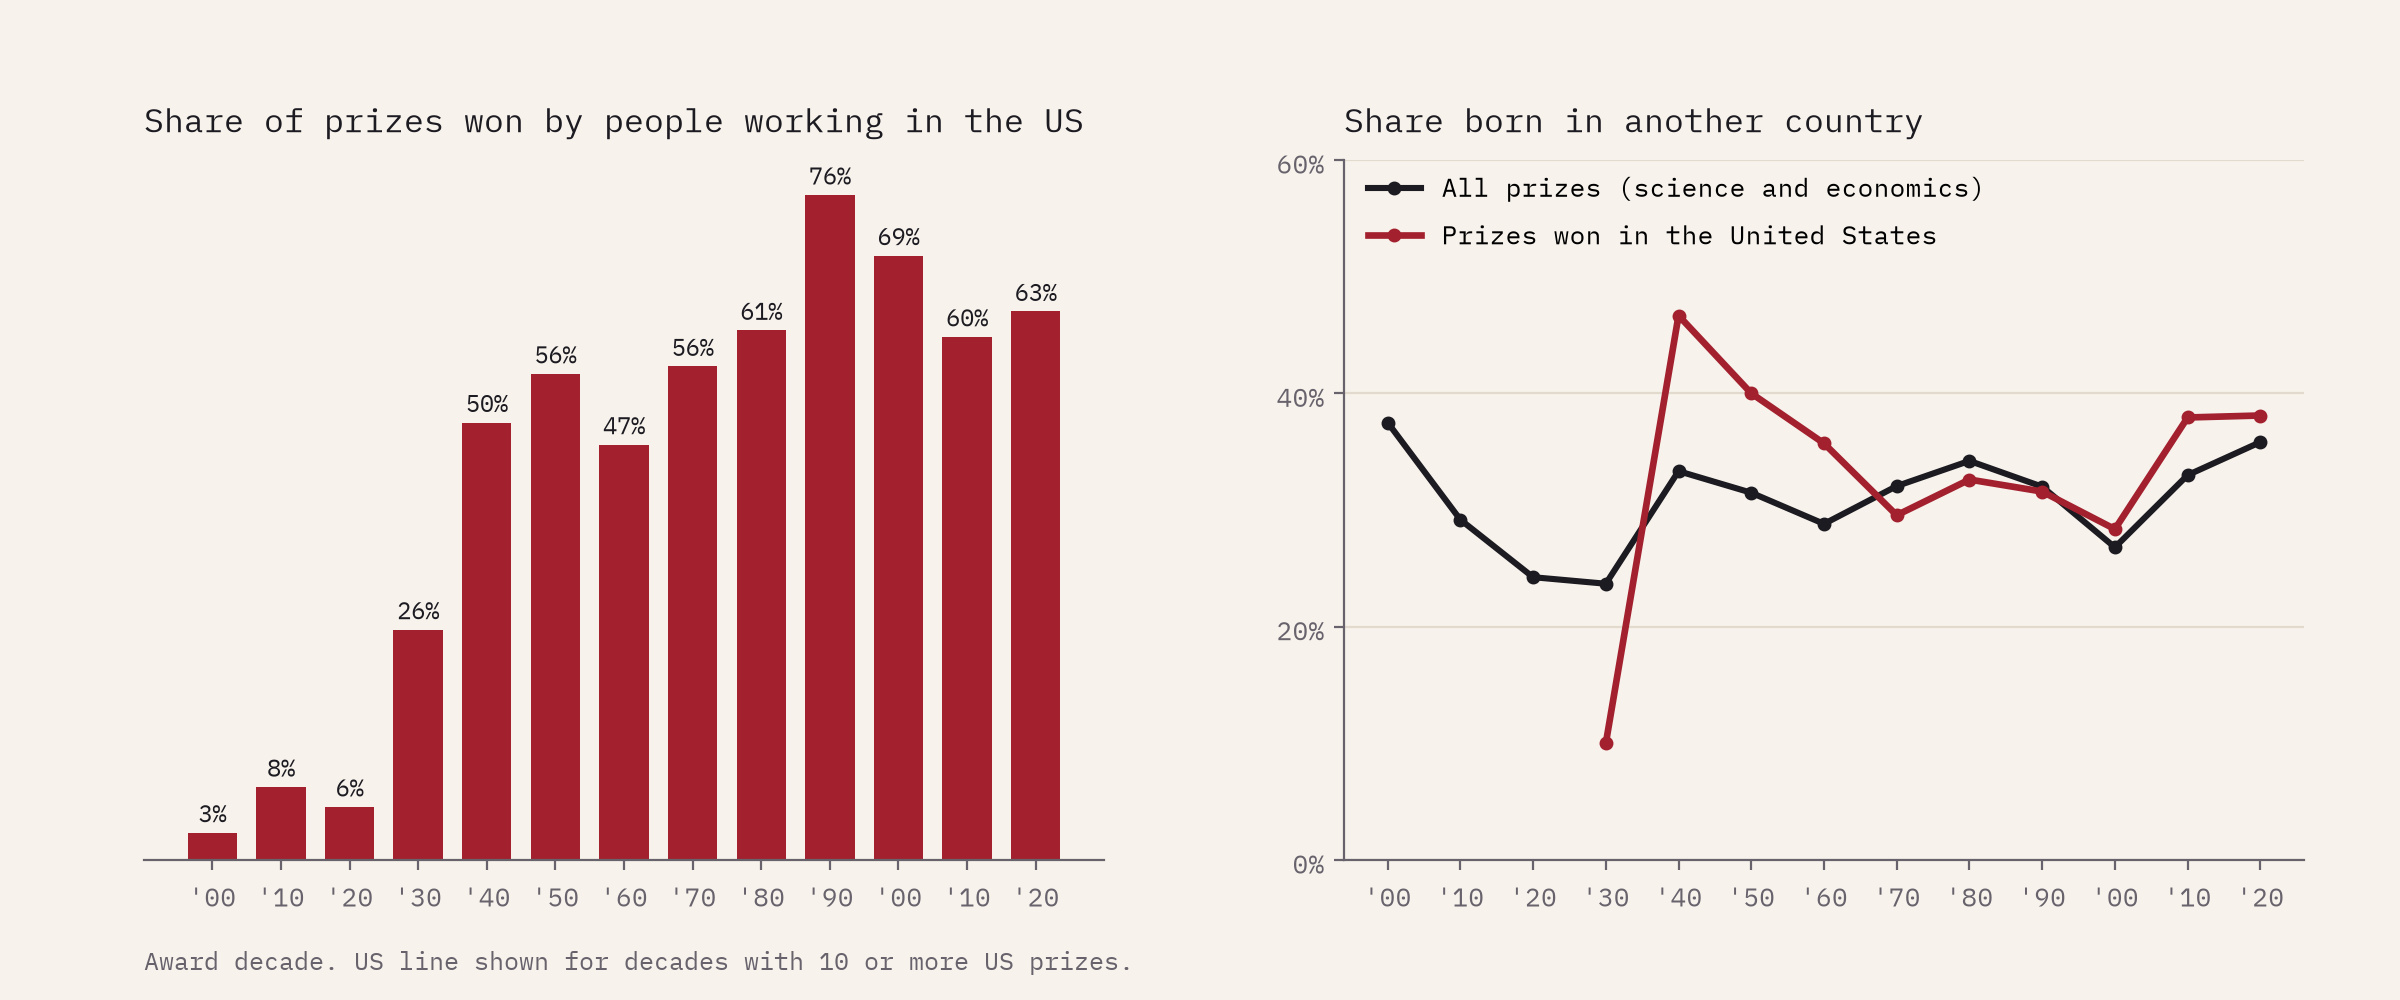
\includegraphics[width=\textwidth]{f_us.png}
\caption{Left: share of each decade's prizes won by people working in the United States. Right: share born in another country, for all prizes and for prizes won in the United States.}\label{fig:us}\end{figure}

\subsection{Germany before and after 1933}
Up to 1932, 31 of 99 prizes (31.3\%) went to people working in Germany; since 1933, 6.5\% (Figure~\ref{fig:germany}). Among the 93 laureates born in the German lands of the day, 10.0\% of those who won up to 1932 (30) were working abroad, against 49.2\% of those who won from 1933 (63). By birth cohort, the share working abroad rises from 14.8\% for those born before 1880 to 37.0\% for those born 1880 to 1909 and 61.5\% for those born 1910 to 1929. 18 German-born laureates born 1880 to 1929 won abroad (Table~\ref{tab:germany}), 10 in the United States and 4 in Britain. They include well-known refugees from Nazi Germany, but the data do not record when or why anyone moved, and the list also includes people who emigrated as children or after the war.

\begin{figure}[tbp]\centering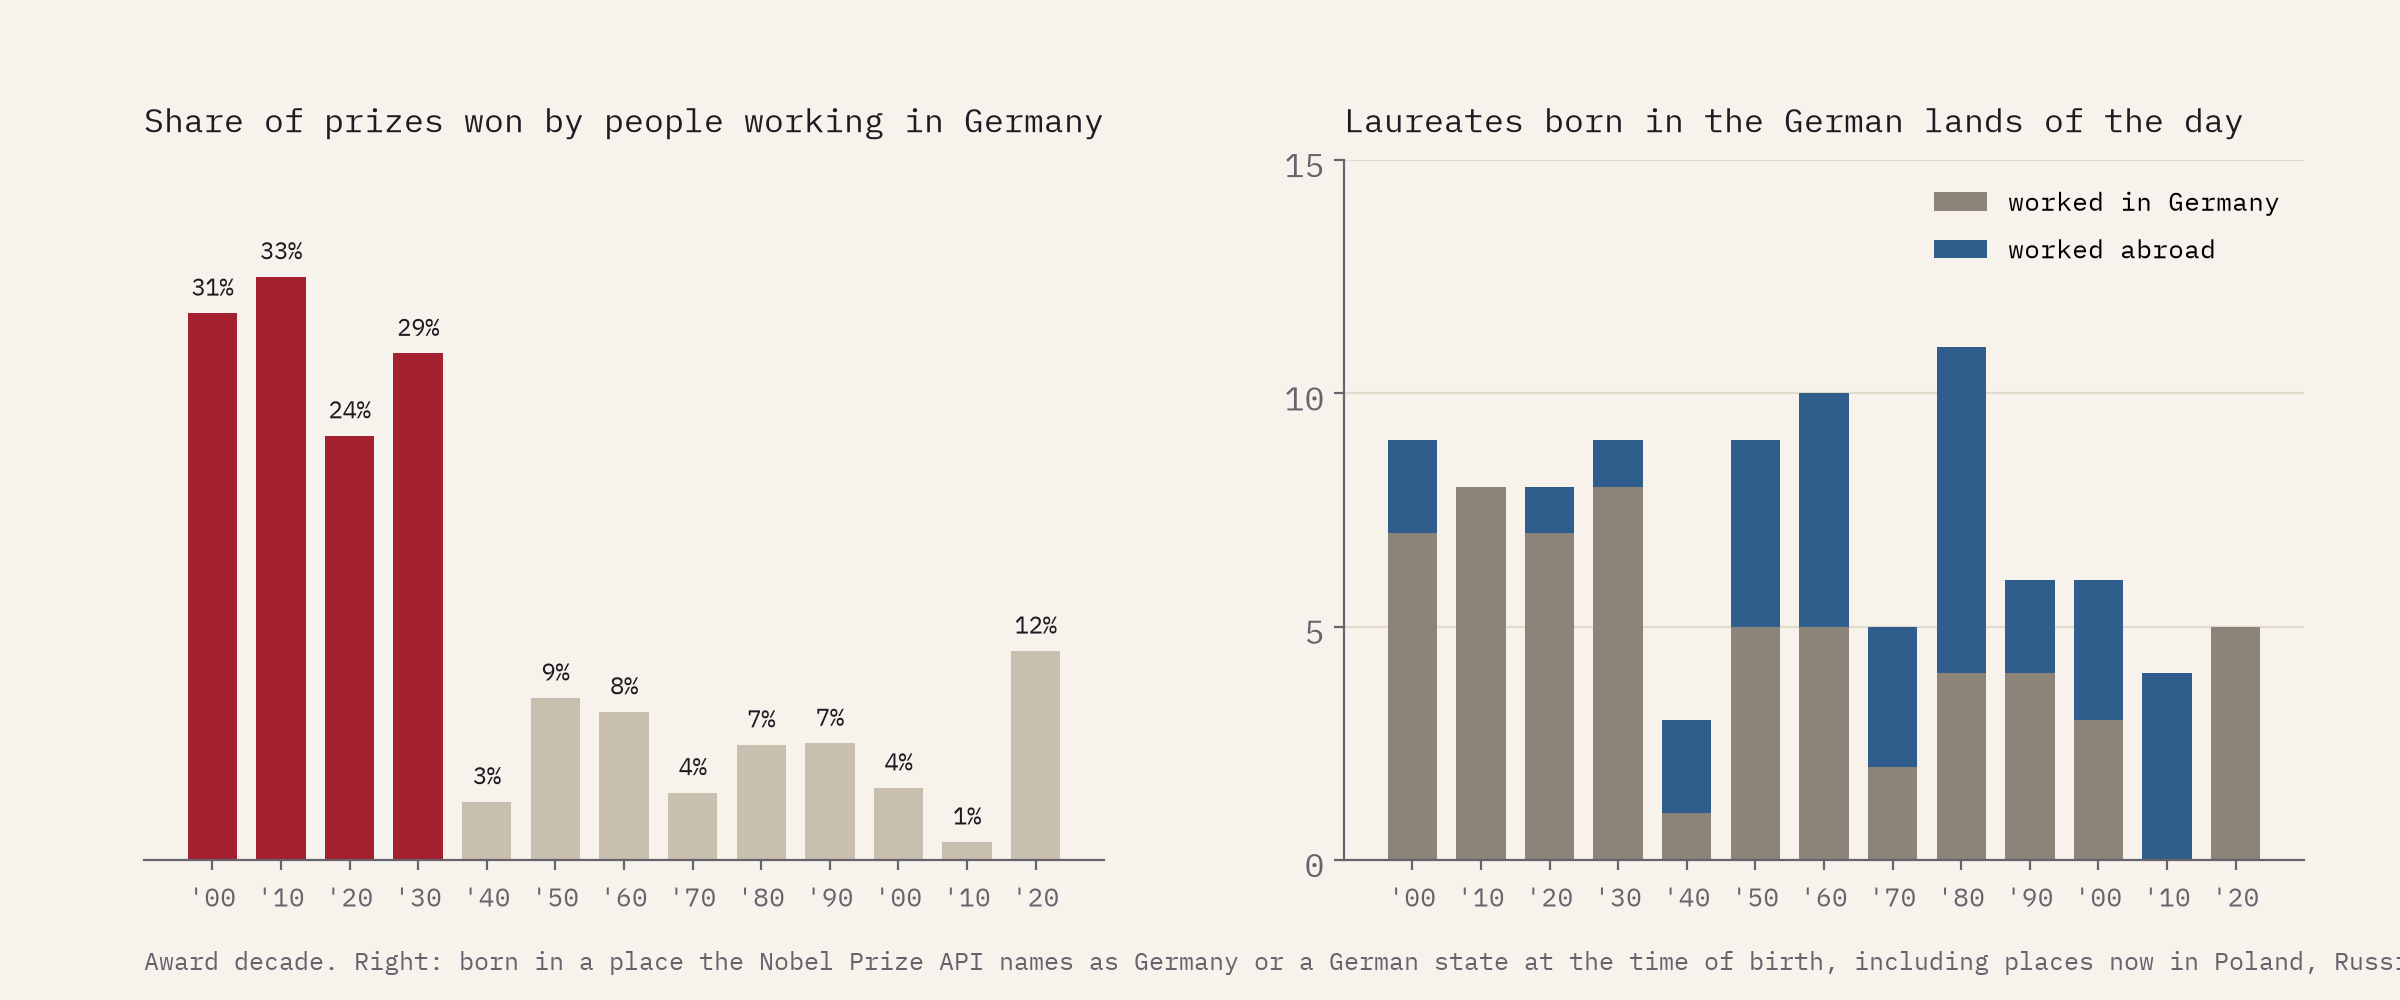
\includegraphics[width=\textwidth]{f_germany.png}
\caption{Left: share of each decade's prizes won by people working in Germany. Right: laureates born in the German lands of the day, by where they won.}\label{fig:germany}\end{figure}

\begin{table}[tbp]\centering\small\caption{German-born laureates (German lands of the day) born 1880 to 1929 who won while working abroad.}\label{tab:germany}\begin{tabular}{lllp{5.4cm}}\toprule Laureate & Born & Prize & Affiliation at the award\\\midrule
Otto Stern & 1888, Sorau & Physics 1943 & Carnegie Institute of Technology, United States\\
Ernst B. Chain & 1906, Berlin & Medicine 1945 & University of Oxford, United Kingdom\\
Fritz Lipmann & 1899, Koenigsberg & Medicine 1953 & Harvard Medical School, United States\\
Hans Krebs & 1900, Hildesheim & Medicine 1953 & Sheffield University, United Kingdom\\
Max Born & 1882, Breslau & Physics 1954 & Edinburgh University, United Kingdom\\
Polykarp Kusch & 1911, Blankenburg & Physics 1955 & Columbia University, United States\\
Maria Goeppert Mayer & 1906, Kattowitz & Physics 1963 & University of California, United States\\
Konrad Bloch & 1912, Neisse & Medicine 1964 & Harvard University, United States\\
Alfred Kastler & 1902, Guebwiller & Physics 1966 & École Normale Supérieure, France\\
Hans Bethe & 1906, Strasbourg & Physics 1967 & Cornell University, United States\\
Max Delbrück & 1906, Berlin & Medicine 1969 & California Institute of Technology (Caltech), United States\\
Sir Bernard Katz & 1911, Leipzig & Medicine 1970 & University College, United Kingdom\\
Gerhard Herzberg & 1904, Hamburg & Chemistry 1971 & National Research Council of Canada, Canada\\
John C. Polanyi & 1929, Berlin & Chemistry 1986 & University of Toronto, Canada\\
Jack Steinberger & 1921, Bad Kissingen & Physics 1988 & CERN, Switzerland\\
Hans G. Dehmelt & 1922, Görlitz & Physics 1989 & University of Washington, United States\\
Herbert Kroemer & 1928, Weimar & Physics 2000 & University of California, United States\\
John B. Goodenough & 1922, Jena & Chemistry 2019 & University of Texas, United States\\
\bottomrule\end{tabular}\end{table}

\subsection{Japan}
Japan's first laureate was Hideki Yukawa in 1949. Japan had 5 science laureates before 2000 and 22 since (Figure~\ref{fig:japan}); since 2000 it is the third most common birth country, with 8.4\% of prizes, against 1.0\% before. 7 of 27 Japanese-born laureates won in the United States; the rest won in Japan, at universities and at companies. Yukawa illustrates the limits of affiliation at the award: his meson theory was developed in Japan, but the API lists Columbia University first in 1949.

\begin{figure}[tbp]\centering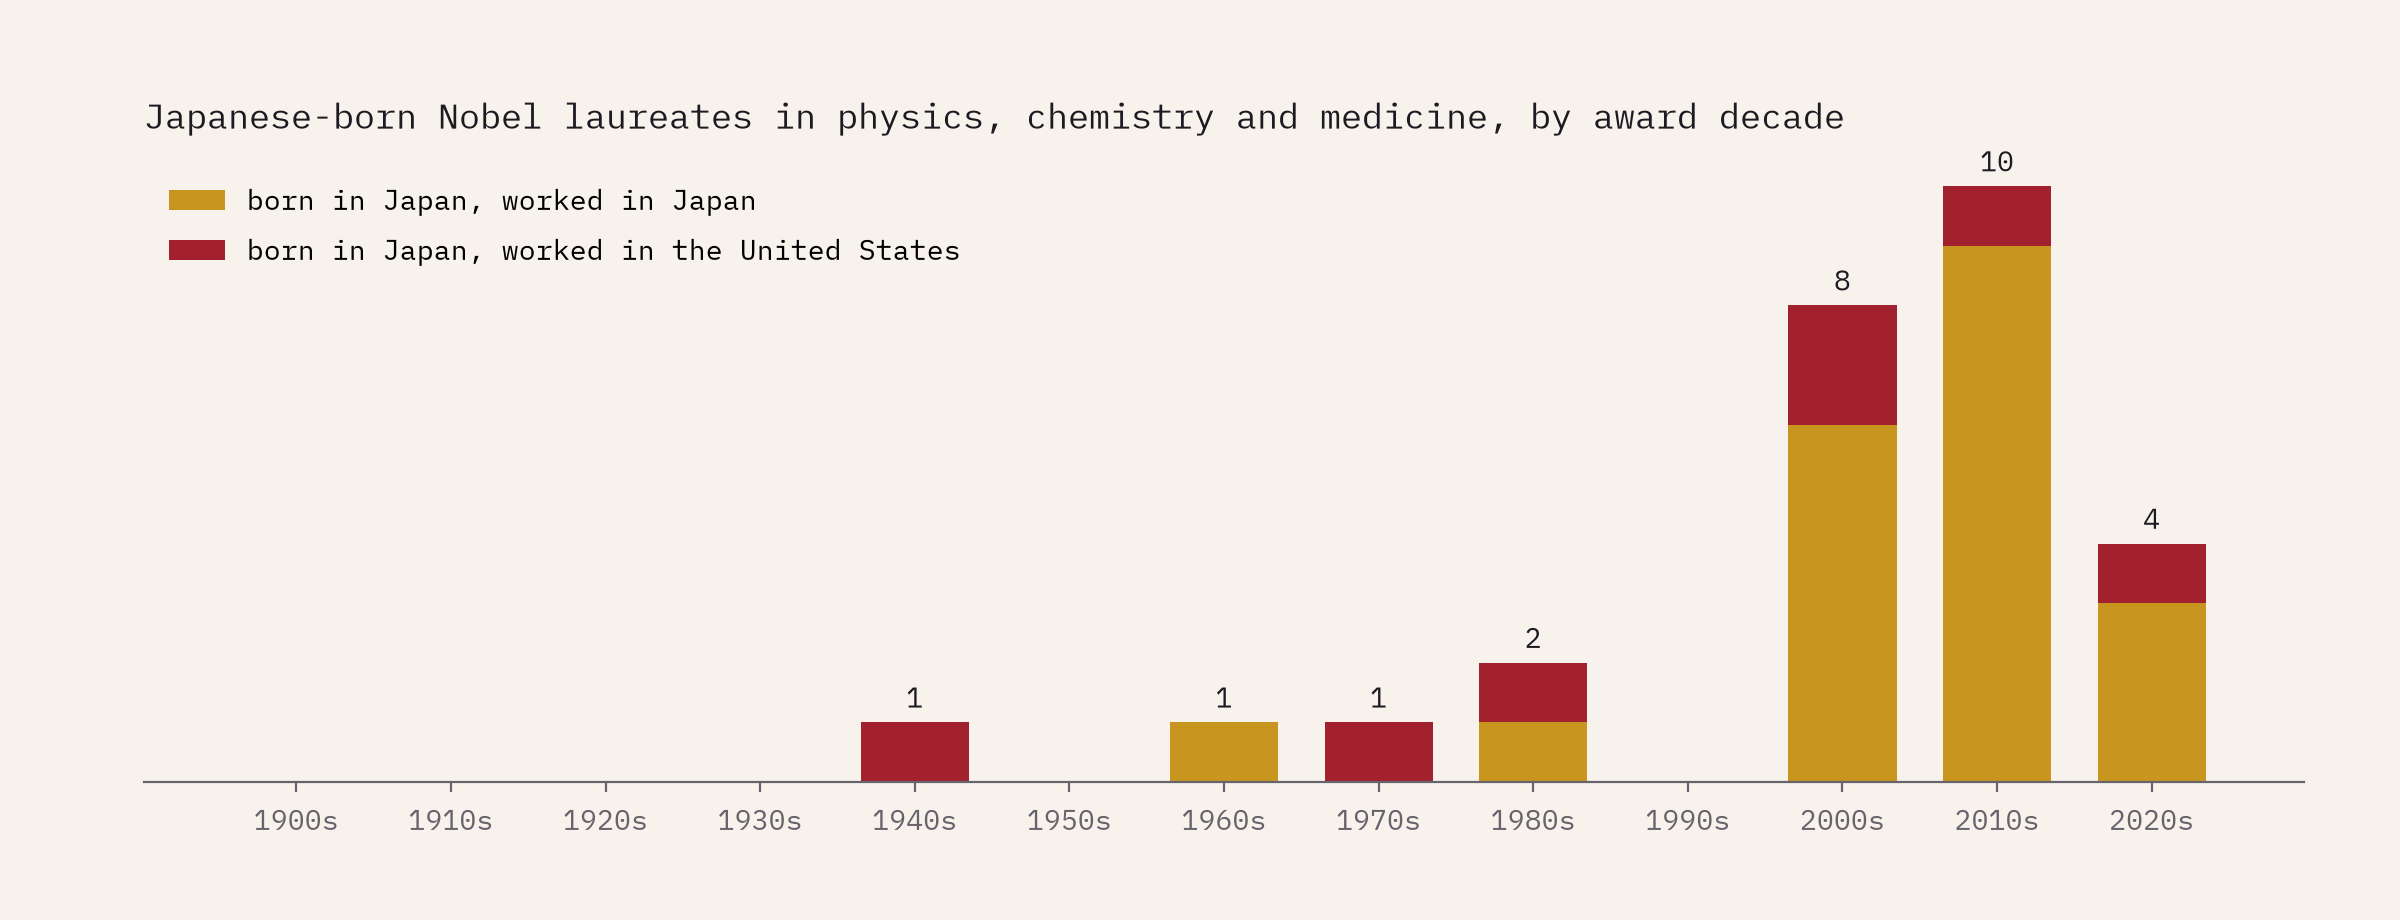
\includegraphics[width=\textwidth]{f_japan.png}
\caption{Japanese-born laureates by award decade and where they were working.}\label{fig:japan}\end{figure}

\subsection{Institutions}
Counting every listed affiliation, the leading institutions are Harvard University (31), MIT (25), Stanford (24) and the University of California, Berkeley (23); 9 of the top ten are American (Figure~\ref{fig:uni}). Max Planck and Kaiser Wilhelm institutes together appear in 30 records. The counts agree exactly with Wikipedia's list for 15 of its top 20 institutions (Table~\ref{tab:wiki}); the rest differ by recent prizes or naming choices.

\begin{figure}[tbp]\centering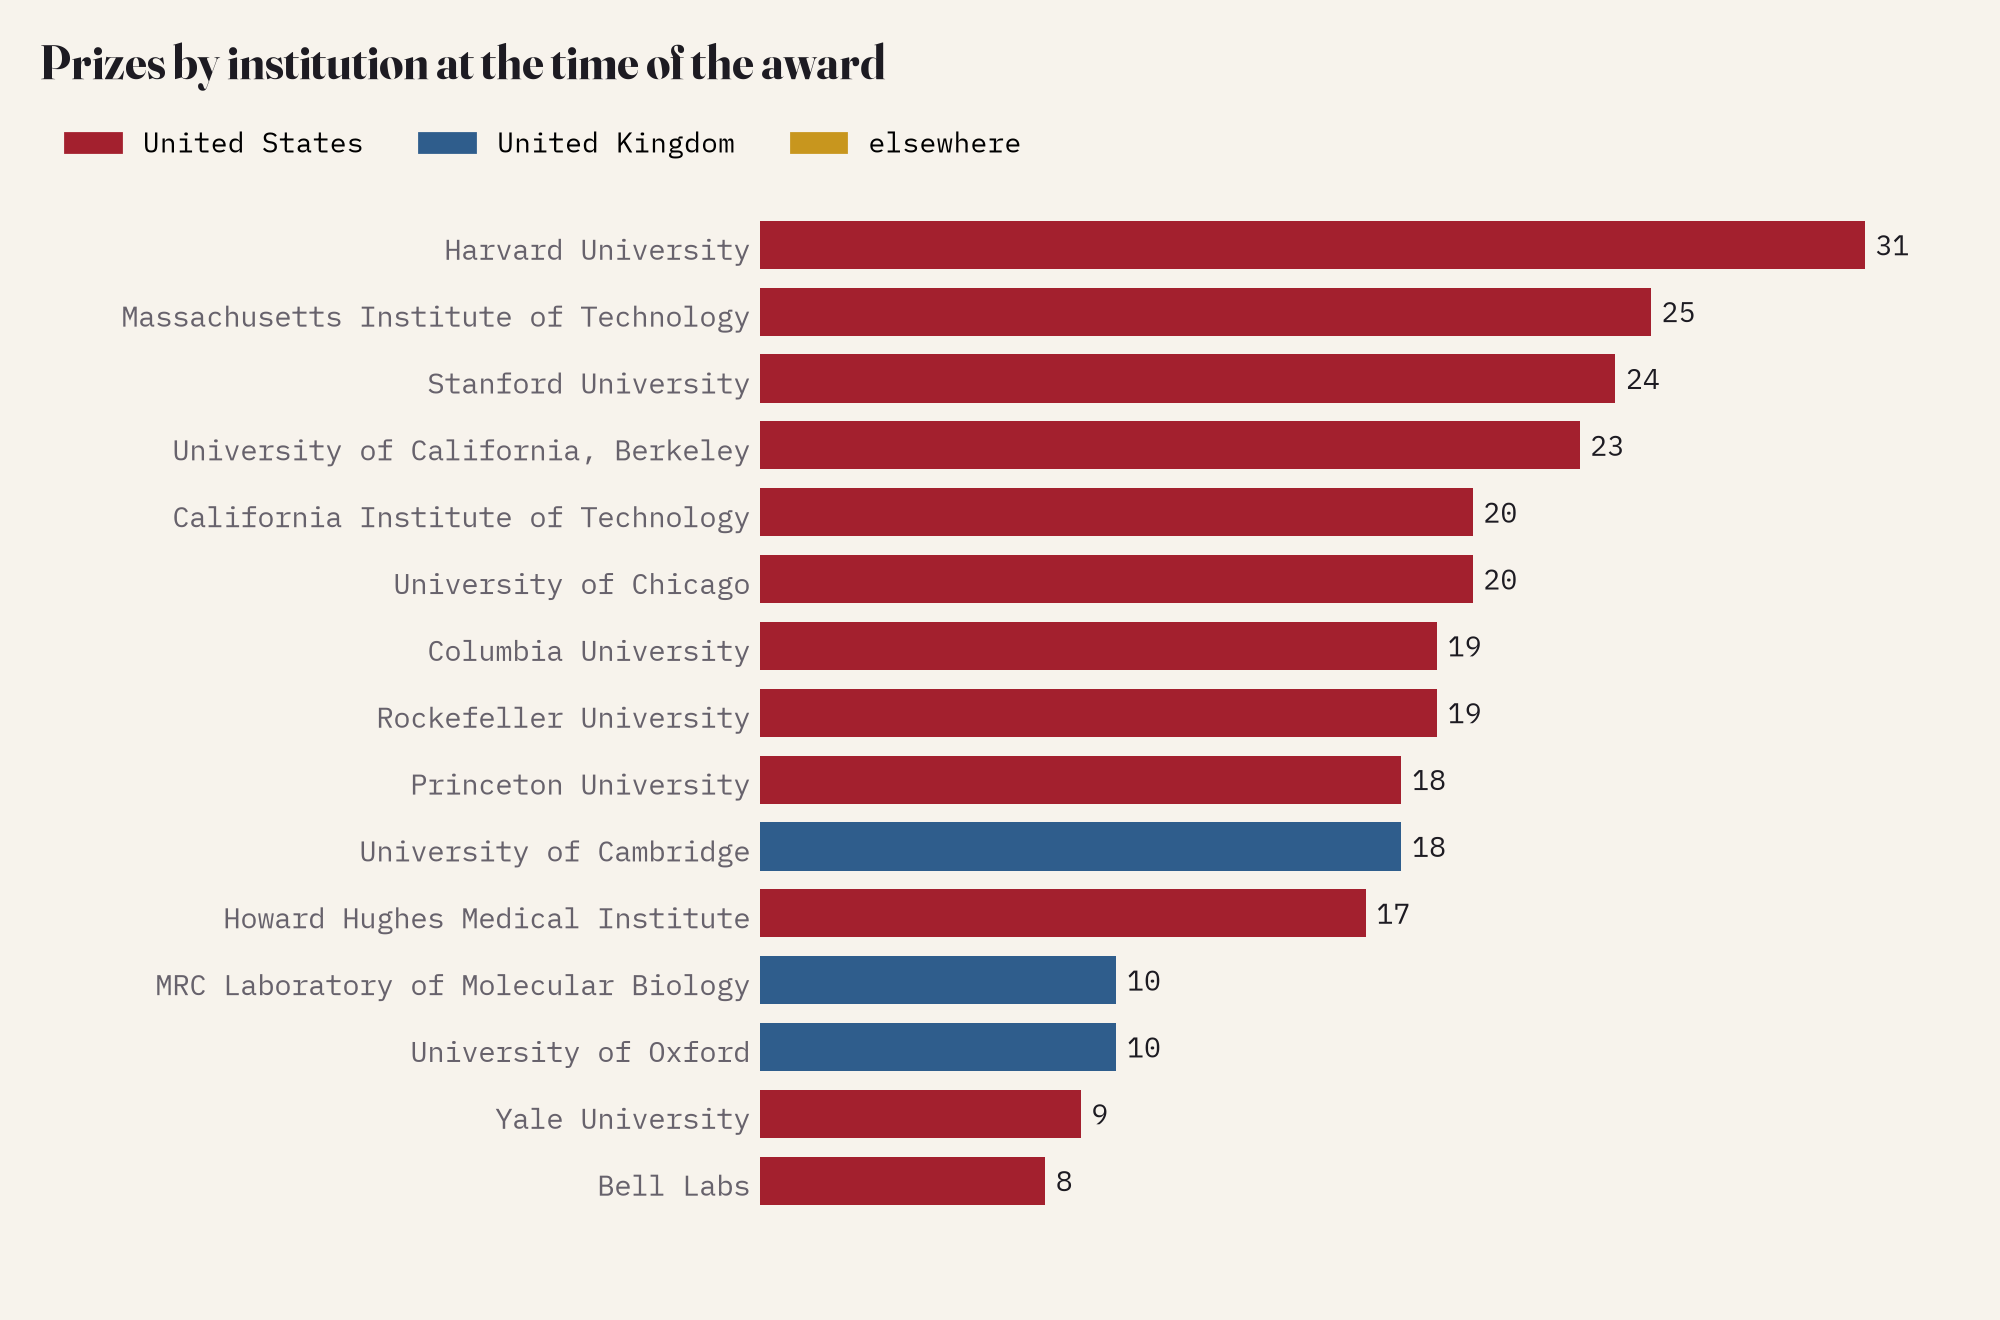
\includegraphics[width=.86\textwidth]{f_universities.png}
\caption{Prizes by institution at the time of the award (every listed affiliation counts).}\label{fig:uni}\end{figure}

\begin{table}[tbp]\centering\small\caption{Institution counts compared with Wikipedia's list (top 20 there).}\label{tab:wiki}\begin{tabular}{lrr}\toprule Institution (Wikipedia name) & Wikipedia & This study\\\midrule
Harvard University & 29 & 31\\
Massachusetts Institute of Technology & 25 & 25\\
Stanford University & 24 & 24\\
University of California, Berkeley & 23 & 23\\
California Institute of Technology & 20 & 20\\
University of Chicago & 20 & 20\\
Columbia University & 19 & 19\\
University of Cambridge & 18 & 18\\
Princeton University & 18 & 18\\
Howard Hughes Medical Institute & 15 & 17\\
Rockefeller University & 13 & 19\\
University of Oxford & 10 & 10\\
MRC Laboratory of Molecular Biology & 10 & 10\\
Yale University & 9 & 9\\
Bell Labs & 8 & 8\\
Cornell University & 8 & 8\\
Harvard Medical School & 8 & 8\\
Case Western Reserve University & 7 & not matched\\
Heidelberg University & 7 & 7\\
University of California, Santa Barbara & 7 & 8\\
\bottomrule\end{tabular}\end{table}

\subsection{Women}
Women received 70 of 1,005 prizes to people (7.0\%): 12 of 314 before 1960 and 40 of 318 since 2000 (Figure~\ref{fig:women}). In the four sciences the share rose from 2.2\% before 2000 to 7.2\% since. Physics has 5 women among 231 laureates, chemistry 8 of 202, medicine 14 of 235, economics 3 of 101, literature 19 of 123 and peace 21 of 113. Women in the flow analysis were born abroad about as often as men (27.6\% of 29 against 31.3\%).

\begin{figure}[tbp]\centering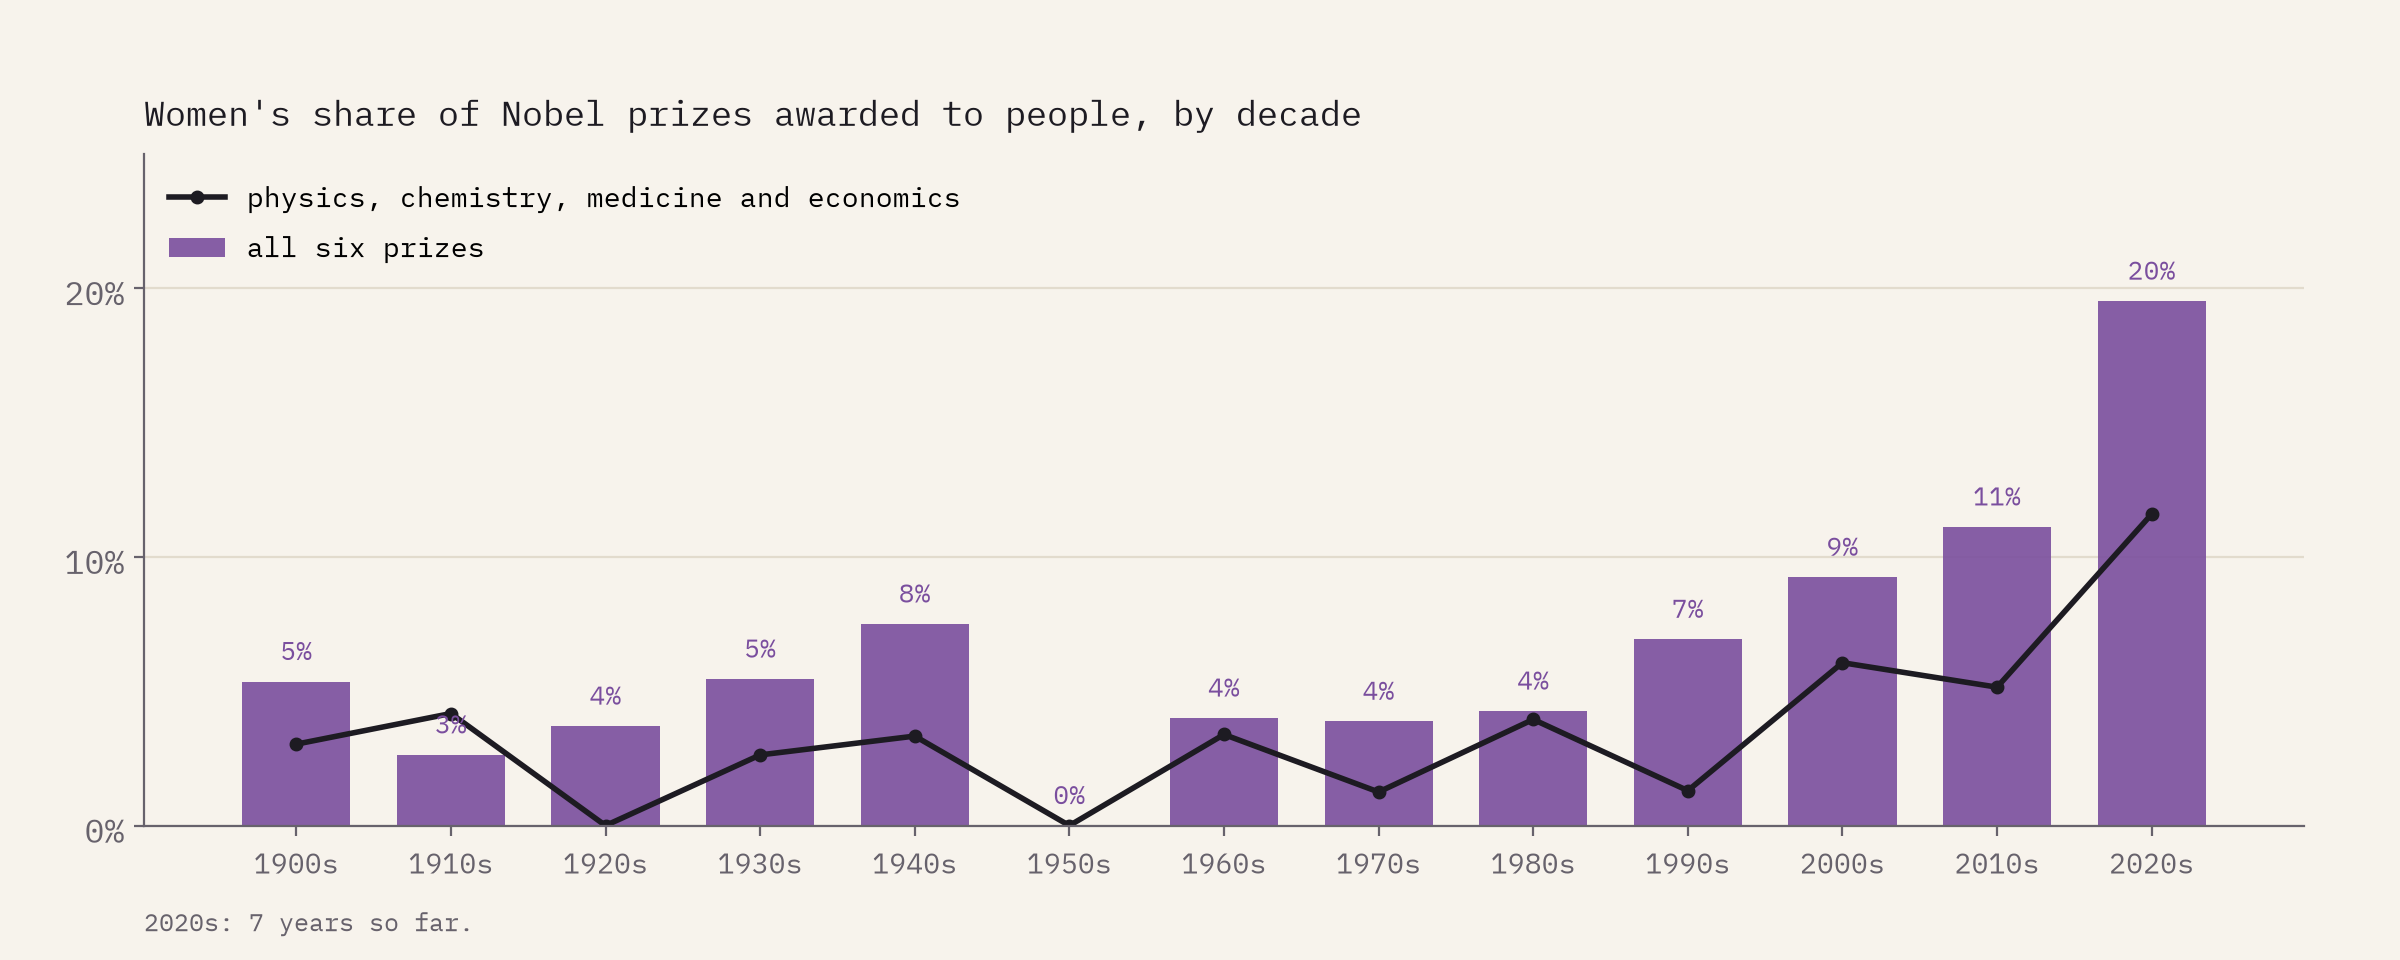
\includegraphics[width=\textwidth]{f_women.png}
\caption{Women's share of prizes to people by decade: all six prizes and the four with affiliations.}\label{fig:women}\end{figure}

\subsection{Born abroad over time}
The share born abroad (Table~\ref{tab:decades}) was 37.5\% in the 1900s, lowest in the 1930s (23.7\%), highest in the 1900s (37.5\%) and 35.8\% in the 2020s so far. The stability of the share hides a change of direction: early moves were mostly between European countries, later ones mostly to the United States.

\begin{table}[tbp]\centering\small\caption{By award decade: records in the flow analysis, share born abroad, share won in the United States and the foreign-born share of those; prizes to people of all six kinds and the share won by women.}\label{tab:decades}\begin{tabular}{lrrrrrr}\toprule Decade & Flow & Born abroad & In US & US born abroad & All prizes & Women\\\midrule
1900s & 32 & 37.5\% & 3.1\% &  & 56 & 5.4\%\\
1910s & 24 & 29.2\% & 8.3\% &  & 38 & 2.6\%\\
1920s & 33 & 24.2\% & 6.1\% &  & 54 & 3.7\%\\
1930s & 38 & 23.7\% & 26.3\% & 10.0\% & 55 & 5.5\%\\
1940s & 30 & 33.3\% & 50.0\% & 46.7\% & 40 & 7.5\%\\
1950s & 54 & 31.5\% & 55.6\% & 40.0\% & 71 & 0.0\%\\
1960s & 59 & 28.8\% & 47.5\% & 35.7\% & 75 & 4.0\%\\
1970s & 78 & 32.0\% & 56.4\% & 29.6\% & 103 & 3.9\%\\
1980s & 76 & 34.2\% & 60.5\% & 32.6\% & 94 & 4.3\%\\
1990s & 75 & 32.0\% & 76.0\% & 31.6\% & 101 & 6.9\%\\
2000s & 97 & 26.8\% & 69.1\% & 28.4\% & 119 & 9.2\%\\
2010s & 97 & 33.0\% & 59.8\% & 37.9\% & 117 & 11.1\%\\
2020s & 67 & 35.8\% & 62.7\% & 38.1\% & 82 & 19.5\%\\
\bottomrule\end{tabular}\end{table}

\subsection{Peace and Literature}
The API gives a country of residence at the award for 224 of 236 Peace and Literature laureates. 18.3\% of them lived outside their birth country: 23.3\% of writers and 13.0\% of peace laureates.

\section{Discussion}
The results restate familiar history in a single, open dataset. Before the 1930s the Nobel map was European and largely German, and movement was mostly between European countries. After 1933 the centre moved to the United States, which since 1950 has hosted most prizes and drawn a third of its laureates from abroad. The German loss appears in the prize record only years later, because prizes typically reward work done long before. Japan stands out as a large late riser that has kept most of its laureates.

The net balance is sensitive to definitions. On present-day borders Germany balances and Poland loses heavily, but most of Poland's loss is Germans born in Silesia and Pomerania. On the API's first affiliation, a laureate holding posts in two countries counts once, though only 19 records are affected.

\section{Limitations}
First, affiliation at the award is not the place of the prize-winning work, which may be decades earlier. Second, birth country is not nationality or the country of education; many laureates born abroad moved as children. Third, present-day borders reassign historical births. Fourth, the Nobel prizes are a small and selective sample whose committees have their own geographic and gender biases, so the results describe the prize record, not science as a whole. Fifth, placement points are approximate where they fall back to city or country centres, although this affects maps, not country counts. Finally, the API's licence could not be confirmed from the downloaded file.

\section{Conclusion}
Two open sources are enough to map where every Nobel laureate was born and where they won, and to show that the prize record has one great importer, the United States, and many exporters. The data, code and interactive map are released for reuse and checking.

\section*{Data and code availability}
The interactive map is at \url{https://maps.tristanhotham.com/nobel-brain-drain/}. Data and code are at \url{https://github.com/Tristan-Hotham/nobel-brain-drain} and archived with this paper at https://doi.org/10.5281/zenodo.23857487. Derived data, text and figures are released under CC BY 4.0 and code under the MIT licence; Wikidata is CC0, and reuse of the laureate list should follow the Nobel Prize API terms.

\section*{AI statement}
I wrote the text, with drafting and editing assistance from Claude (Anthropic), which also helped prepare the analysis code. I reviewed and checked all text and results.

\begin{thebibliography}{9}
\bibitem[Bast and Buchhold(2017)]{qlever} Bast, H. and Buchhold, B. (2017) QLever: a query engine for efficient SPARQL+text search. \emph{Proceedings of the 2017 ACM Conference on Information and Knowledge Management}, 647 to 656.
\bibitem[Medawar and Pyke(2001)]{medawar} Medawar, J. and Pyke, D. (2001) \emph{Hitler's Gift: Scientists who Fled Nazi Germany}. London: Richard Cohen Books.
\bibitem[Natural Earth(2026)]{naturalearth} Natural Earth (2026) Admin 0 countries and populated places. Public domain. \url{https://www.naturalearthdata.com/}
\bibitem[Nobel Prize Outreach(2026)]{nobelapi} Nobel Prize Outreach (2026) Nobel Prize API, version 2.1. \url{https://api.nobelprize.org/}
\bibitem[Schlagberger et al.(2016)]{schlagberger} Schlagberger, E. M., Bornmann, L. and Bauer, J. (2016) At what institutions did Nobel laureates do their prize-winning work? An analysis of biographical information on Nobel laureates from 1994 to 2014. \emph{Scientometrics}, 109, 723 to 767.
\bibitem[Vrandečić and Krötzsch(2014)]{wikidata} Vrandečić, D. and Krötzsch, M. (2014) Wikidata: a free collaborative knowledgebase. \emph{Communications of the ACM}, 57(10), 78 to 85.
\bibitem[Zuckerman(1977)]{zuckerman} Zuckerman, H. (1977) \emph{Scientific Elite: Nobel Laureates in the United States}. New York: Free Press.
\end{thebibliography}
\end{document}
